\begin{figure*}[!tb]
  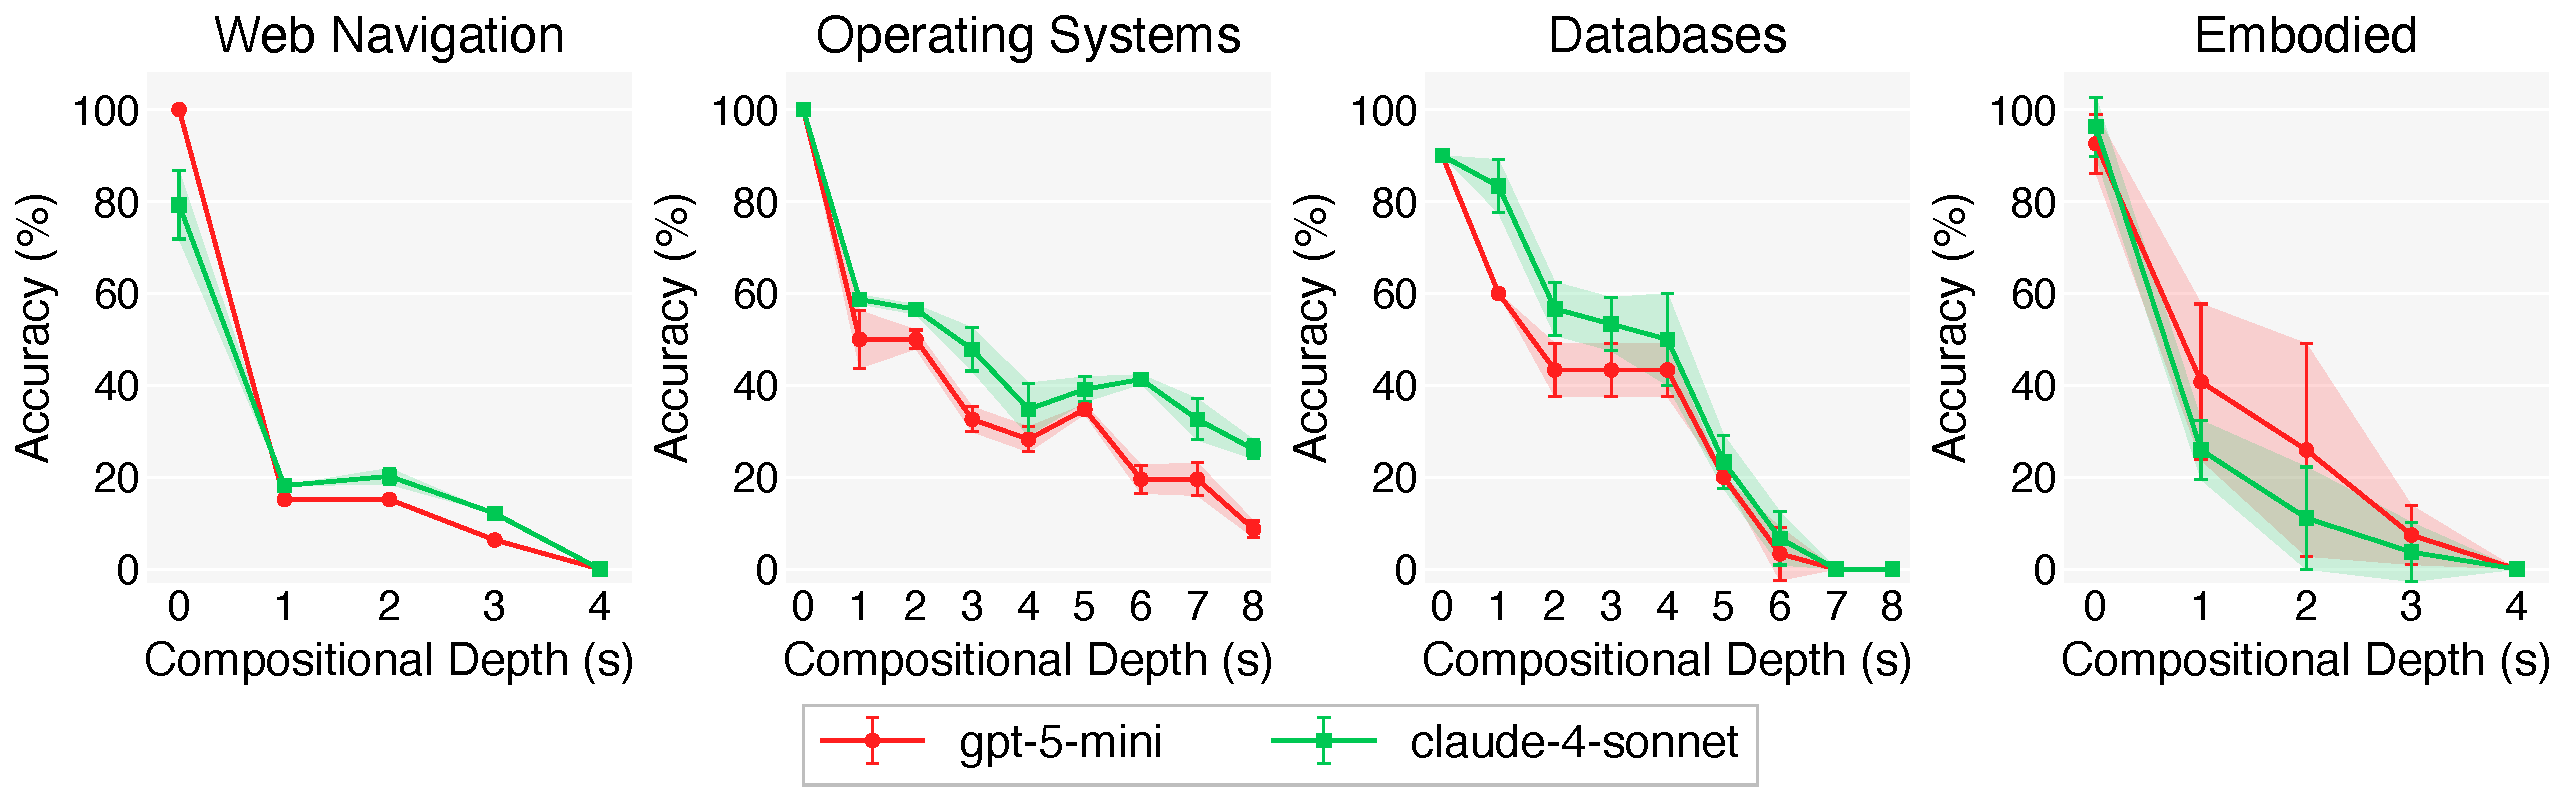
\includegraphics[width=\textwidth]{horizon_4panel.pdf}
  \centering
   % \caption{\textit{Current model performance as a function of horizon extension.} Plots show success rate (accuracy) versus the compositional depth $s$, where $s$ denotes the \texttt{HORIZON}-defined extension level corresponding to the number of high-level subtasks composed within a task. Accuracy is computed over task sets with the same $s$. Each point reports the mean over three independent runs with identical task sets; variability across runs is shown as $\pm$ one standard deviation (error bars). We evaluate GPT-5-mini and Claude-4-Sonnet across all domains. Across models and domains, performance consistently decreases and exhibits a sharp drop beyond a certain value of $s$, empirically supporting the validity of our horizontal horizon definition. More details are provided in Section~\ref{sec:5}.}
   \caption{\textit{Current model performance as a function of horizon extension.} Plots show success rate (accuracy) versus the compositional depth $s$, where $s$ denotes the \texttt{HORIZON}-defined extension level corresponding to the number of high-level subtasks composed within a task. Note that $s$ measures compositional depth, not raw action count. Each unit of $s$ expands to multiple low-level actions during execution, with per-trajectory action budgets of max 150 (Web), 50 (OS), 31 (DB), and 34 (Embodied) steps. Accuracy is computed over task sets with the same $s$. Each point reports the mean over three independent runs with identical task sets; variability across runs is shown as $\pm$ one standard deviation (error bars). We evaluate GPT-5-mini and Claude-4-Sonnet across all domains. Across models and domains, performance consistently decreases and exhibits a sharp drop beyond a certain value of $s$, empirically supporting the validity of our horizontal horizon definition. More details are provided in Section~\ref{sec:5}.}
  \label{fig:horizon}
%   \vspace{-6pt}
\end{figure*}